% <<FF>> ***********************************************************************
% https://www.overleaf.com/learn/latex/Beamer_Presentations:_A_Tutorial_for_Beginners_(Part_2)%E2%80%94Lists,_Columns,_Pictures,_Descriptions_and_Tables#The_Description_Environment
\section{Simple Example}
\begin{frame}
  \frametitle{A motivating Example for SMC}

 % This example is taken from \cite{utkin2020}.
  
 \begin{columns}
   \column{0.5\textwidth} % ************************

   \begin{example}
     Sliding mode of the system \cite{utkin2020}:

      \begin{equation}
         \ddot x = \sin(3 t) + u 
       \end{equation}
       with sliding surface
       \begin{equation}
        s = c \dot x + x
       \end{equation}
       with control law
       \begin{equation}
         u = -M \sgn(s)
       \end{equation}
    \end{example}   
     \column{0.5\textwidth} % ************************
   \centering
   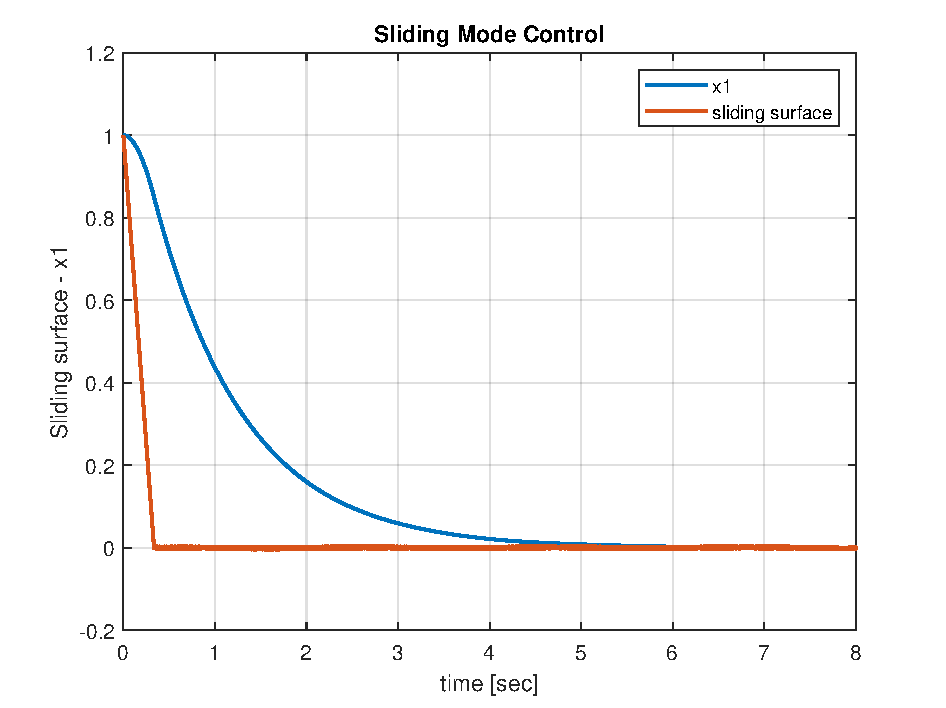
\includegraphics[height=4cm]{./pictures/SMCutkinRoadmap.pdf}
   Simulation results for $M = 3$ \\ and $c = 1\; \unit{s}^{-1}$
\end{columns}

\vspace*{2mm}

% \begin{block}{Remark}
  If the system is in sliding mode, \ie. $s=0$, the dynamics is
  $s = \dot x + x =0$ and therefore indepentend of system
  parameters or disturbance $\leadsto$ robust !
% \end{block}

\end{frame}

% <<FF>> *************************************************************

 \begin{frame}
\frametitle{Sample frame title}

In this slide, some important text will be
\alert{highlighted} because it's important.
Please, don't abuse it.

\begin{block}{Remark}
Sample text
\end{block}

\begin{alertblock}{Important theorem}
Sample text in red box
\end{alertblock}

\begin{examples}
Sample text in green box. The title of the block is ``Examples".
\end{examples}
\end{frame}




 
%%% Local Variables:
%%% mode: latex
%%% TeX-master: "SMC4Students"
%%% End:
